\documentclass[fleqn,10pt]{olplainarticle}
% Use option lineno for line numbers 

\title{Example Article Title}

\author[1]{Jakob Reinhardt}
\affil[1]{Yale University}


\begin{document}

\setlength{\parindent}{0pt}
\flushbottom
\thispagestyle{empty}

\section*{Setup}

Households have quasi-linear preferences over consumption $c$ and leisure $l$. They are indexed by their latent wage $\omega \sim F$, which is continuously distributed over $\left[\underline{\omega}, \overline{\omega}\right]$. Depending on which jurisdiction $j \in \{1, \ldots, J\} \equiv \left[J\right]$ they reside in, they face a jurisdiction-specific tax-and transfer system consisting of a linear tax $\tau_j$ and a transfer $T_j$. Defining disposable income as $y = wl$ we can write the consumer's choice problem as:

$$\max_{c, y, j \in \left[ J\right]} c - k(\frac{y}{\omega}) \;\;\;s.t. \;\; c \leq T_j + (1-\tau_j)y$$

where $k(\cdot)$ is the differentiable, increasing and convex cost of supplying labor with $k^\prime(0) = 0$. Given a consumer chooses to live in jurisdiction $j$, denoted $J(\{\tau_j, T_j\}_{j \in \left[J\right]}, \omega) = j$, she will choose $y^*(\tau_j, \omega)$ satisfying: 

$$(1-\tau_j) = \frac{1}{\omega}k^\prime(\frac{y^*}{\omega})$$

We know $\frac{\partial y^*}{\partial \tau_j}(\tau_j, \omega) \equiv y^*_\tau(\tau_j, \omega) \leq 0$ and by convexity $\frac{\partial y^*}{\partial \omega}(\tau_j, \omega) \equiv y^*_\omega(\tau_j, \omega) \geq 0$. Households achieve indirect utility $v(\tau_j, T_j, \omega)$ if choosing jurisdiction $j$.\\
Household indifference curves in the $(\tau_j, T_j)$-space are upwards sloping with slope of $y^*(\tau_j, \omega)$. From $y_\omega(\tau_j, \omega) \geq 0$ we can conclude that higher types have steeper indifference curves, implying the Spence-Mirrlees single-crossing condition is satisfied. 

\section*{Equilibrium}
Given a set of taxes and transfers $\{\tau_j, T_j\}_{j\in \left[J\right]}$, an equilibrium is an allocation $\{c(\omega), y(\omega), J(\omega)\}$ such that:
\begin{enumerate}
    \item Households choose optimally, i.e. for each $\omega$ the bundle $(c, y, J)$ solves 
            \begin{equation} \label{y_FOC}
                (1-\tau_J) = \frac{1}{\omega}k^\prime(\frac{y}{\omega})
            \end{equation}
            \begin{equation} \label{c_FOC}
                c = T_J + (1-\tau_J)y
            \end{equation}
            \begin{equation} \label{j_choice}
                v(\tau_J, T_J, \omega) \geq v(\tau_{j}, T_{j}, \omega)  \;\;\;\forall j \in \left[J\right]
            \end{equation}
    \item Population in each jurisdiction is non-zero and each jurisdiction's budget is balanced:
        \begin{equation} \label{positive_pop}
            \int\mathbb{I}_{J(\omega) = j} \;dP_F > 0 \;\;\;\forall j \in \left[J\right]
        \end{equation}
        \begin{equation} \label{budget_balance}
            \int\left(\tau_jy(\omega) - T_j\right) \mathbb{I}_{J(\omega) = j}  \;dP_F \geq 0 \;\;\;\forall j \in \left[J\right]
        \end{equation}
\end{enumerate}
This is closely related to equilibrium notions of \cite{EppleFilimonRomer1984} and \cite{EppleRomer1991}. However, here we are not restricting the set of tax- and transfer-systems to be in ``political equilibrium''. I think this has the benefit of accommodating a wide range of potential interactions between jurisdictions.

\paragraph{Claim 1: Stratification} Each jurisdiction contains households with types in a single interval. Households are fully stratified by their types, the set of jurisdiction intervals partitions the whole type space  $\left[\underline{\omega}, \overline{\omega}\right]$. \\

This is a simple consequence of preferences being single-crossing in $(\tau_j, T_j)$-space. To show this, we first order the equilibrium tax rates as $\tau_1 < \ldots < \tau_J$. Then we can note that if a type $\omega$ prefers a lower tax jurisdiction $j$ over  a higher tax jurisdiction $j^\prime$, then any type $\omega^\prime > \omega$ also prefers jurisdiction $j$ over $j^\prime$. This can be shown either with simple algebra\footnote{Suppose $v(\tau_j, T_j, \omega) \geq v(t_{j^\prime}, T_{j^\prime}, \omega)$ and $\omega^\prime > \omega$. Then $v(\tau_j, T_j, \omega^\prime) \geq v(t_{j^\prime}, T_{j^\prime}, \omega^\prime)$ follows from applying the definition of $v\left(\cdot\right)$ and the FOC, and then using $\tau_j < \tau_{j^\prime}$,  $y_\omega \geq 0$ and $y_\omega$ being decreasing in $\tau$.} or by plotting the indifference curves of type $\omega$ and $\omega^\prime$ in the $(\tau_j, T_j)$-space through any point. For lower tax rates, the better-than-set of type $\omega$ is a subset of the better-than-set of type $\omega^\prime$, hence if any tax-transfer bundle to the left of $(\tau_j, T_j)$ is preferred by $\omega$, it will also be preferred by $\omega^\prime$.\\

If an equilibrium exists, then by the positive population requirement in (\ref{positive_pop}), we can pick two $\omega$'s for any two ``adjacent'' communities $j$ and $j+1$ such that one prefers the higher-tax jurisdiction and the other prefers the lower-tax one. Because the indirect utility function is continuous by Berge's theorem, there must exist a type $\tilde\omega_j$ which is exactly indifferent between the two ``adjacent'' communities. Hence, any $\omega > \tilde\omega_j$ prefers jurisdiction $j$ over $j+1$, and similarly lower types prefer $j+1$ over $j$. Repeat the same exercise for jurisdictions $j+1$ and $j+2$ and we conclude any $\omega \in \left[\tilde\omega_j, \tilde\omega_{j+1}\right]$ will prefer jurisdiction $j+1$ over all other jurisdictions, since the argument in the previous paragraph did not restrict to ``adjacent'' communities. Thus in equilibrium households will be fully stratified along their types; $$J(\omega) = j \iff \omega \in \left[\tilde\omega_j, \tilde\omega_{j-1}\right]$$
for some $\tilde\omega_J < \ldots < \tilde\omega_0$ where we define $\tilde\omega_0 = \underline{\omega}$ and $\tilde\omega_{J} = \overline{\omega}$.\\

Combining the stratification result with the FOCs in (1) and (2) we have characterized $\{c(\omega), y(\omega), J(\omega)\}$ as a function of $\{\tau_j, T_j\}_{j\in \left[J\right]}$ \textit{if} an equilibrium exists. 

\paragraph{Remark 1:} We have yet to characterize the set of $(\tau, T)$-pairs that form an equilibrium. I don't quite know how to proceed here. I have two hypotheses: First, all tax rates in $(0,1)$ are permissible because by the boundary condition on $k(\cdot)$ even the lowest type will always choose positive income. Second, one can iteratively solve for the desired equilibrium by starting with uniform transfers at first and then updating according to (\ref{budget_balance}).\\

\section{Welfare Analysis}
In this setting, tax competition among jurisdictions lowers the tax rates that jurisdictions can charge, if jurisdiction set tax rates strategically. For example, we could assume that jurisdictions aim to maximize welfare for their constituents. In that case, a marginal tax change would not leave the jurisdiction better of, or formally:


\newpage
One first observation is that taking $\{t_j, T_j\}_{j\in [J]}$ as fixed and assuming $(\tilde\omega_j, \tilde\omega_{j-1})$ are differentiable as functions of $T_j$, we can apply Leibniz' rule to show:
\begin{align*}
    & \int \left(\tau_jy(\omega) - T_j\right) \mathbb{I}_{J(\omega) = j}  \;dP_F  & \geq & \;0 \\
    \iff & \int_{\tilde\omega_j}^{\tilde\omega_{j-1}} \tau_jy(\omega) - T_j  \;dP_F  &  \geq & \;  0 \\
    \implies & \frac{\partial\tilde\omega_{j-1}}{\partial T_j}\left(\tau_j y\left(\tau_j, \tilde\omega_{j-1}\right) - T_j\right) - \frac{\partial\tilde\omega_{j}}{\partial T_j} \left(\tau_j y\left(\tau_j, \tilde\omega_{j}\right) - T_j\right)&  \geq & \; P(J(\omega) = j)
\end{align*}
However, this does not fully characterize the $T_j$'s. First, differentiability of $(\tilde\omega_j, \tilde\omega_{j-1})$ was assumed. Maybe this is straightforward to show, but I don't see how / don't know where to look for some guidance. Second, using Leibniz' rule this way only generates a necessary condition, not a sufficient one (or am I mistaken?). Third, one needs to show a solution to the equation exists. Fourth, even if the two previous concerns could be alleviated, this only characterizes $T_j$ taking $T_{-j}$ as given. In reality, all $T_j$'s are interdependent through the $\tilde\omega_j$'s. This reminds me of a fixed point problem, but I can't quite formalize it.\\

A second attempt is to focus on only two jurisdictions, $J=2$. Then the positive population requirement simplifies if we define $V(\tau_j, \omega)$ as $v(\tau_j, T_j, \omega) - T_j$:
\begin{align*} 
    & \int\mathbb{I}_{J(\omega) = j} \;dP_F > 0 \;\;\;\forall j \in \left[J\right] \\
    \iff & v(\tau_1, T_1, \underline{\omega}) < v(\tau_2, T_2, \underline{\omega}) \text{ and } v(\tau_1, T_1, \overline{\omega}) > v(\tau_2, T_2, \overline{\omega}) \\
    \iff &  V(\tau_1, \overline{\omega}) - V(\tau_2, \overline{\omega})  < T_2 - T_1  < V(\tau_1, \underline{\omega}) - V(\tau_2, \underline{\omega}) 
\end{align*}
Clearly $T_2 > T_1$, in that the households choosing the higher tax jurisdiction have to be compensated. Compensation cannot be so high that even the highest type prefers community 2, and not so low that even the lowest type prefers community 1. When does budget balance follow? We can rearrange the budget balance constraint to:
\begin{align*}
    & T_j \leq \frac{\int_{\tilde\omega_j}^{\tilde\omega_{j-1}} \tau_jy(\tau_j, \omega) \; dP_F}{F(\tilde\omega_{j-1})  - F(\tilde\omega_j)}
\end{align*}
However, $T_j$ appears on both sides of the inequality because the $\tilde\omega_j$ implicitly depend on $T_j$, too. We know $\lim_{T_1 \rightarrow \infty} \tilde\omega_1 = \underline{\omega}$ and similarly for $T_2$ $\tilde\omega_1$ converges to $\overline{\omega}$, since at some transfer high enough everybody will be incentivized to move into each respective jurisdiction. Hence $\tau_j\mathbb{E} \left[ y(\tau_j, \omega) \right]$ is an upper bound for $T_j$ that need not be sharp. Combining these two thoughts, we know the positive population requirement restricts the admissible pairs $(T_1, T_2)$ to be in  a trapezoid
\begin{figure}[htbp]
    \centering
    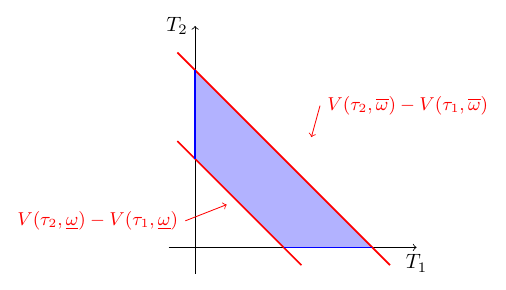
\includegraphics[width=0.7\textwidth]{figures/trapezoid_simple.png}
    \label{fig:trapezoid}
\end{figure}
but we have struggled to make much of the budget balance constraints.\\


\bibliography{sample}



\end{document}



v = T + (1-tau)y - k(y/w)
T1 - T2








